Das Projekt kann in drei Unterprojekte eingeteilt werden. Fsverify, also die Verifizierung selber, verifysetup, ein Programm, um das System richtig zu konfigurieren, um die Nutzung von fsverify möglich zu machen und fbwarn, ein Programm, welches den Nutzer grafisch über eine fehlgeschlagene Verifizierung informiert.

\documentclass[12pt,a4paper]{article}

\usepackage[utf8]{inputenc}
\usepackage[T1]{fontenc}
\usepackage{graphicx}
\usepackage[left=2.50cm, right=2.50cm, top=2.50cm, bottom=2.50cm]{geometry}
\usepackage[german]{babel}
\usepackage{setspace}
\usepackage{tocbibind}
\usepackage{minted}
\usepackage{enumitem}
\usepackage{microtype}
\usepackage{aliascnt,ccaption}
\usepackage[plainpages=false]{hyperref}
\setlist[description]{style=nextline}

\hypersetup{
	colorlinks   = true,    % Colours links instead of ugly boxes
	urlcolor     = cyan,    % Colour for external hyperlinks
	linkcolor    = cyan,    % Colour of internal links
	citecolor    = black      % Colour of citations
}

\newaliascnt{figurealt}{figure}% New alias counter for figure float
\aliascntresetthe{figurealt}
\makeatletter
\renewcommand{\contcaption}{%
  \expandafter\addtocounter\expandafter{\@captype alt}{\m@ne}% Step alias cntr back
  \expandafter\refstepcounter\expandafter{\@captype alt}% Make reference
  \@contcaption\@captype}
\makeatother

\title{fsverify}
\author{-}
\setstretch{1.5}
\begin{document}
\pagenumbering{gobble}
\begin{center}
	{\setstretch{1.0}
		\vspace*{1cm}
		
		\Huge
		\textbf{FsVerify}
		
		\vspace{2cm}
		
		\textbf{Xenia}
		
		\vspace{1.5cm}
		
		Reflexion zum\\
		AP Informatik
		
		\vfill
	}
\end{center}

%%% Local Variables:
%%% mode: latex
%%% TeX-master: "fsverify"
%%% End:

\clearpage
\newpage
\tableofcontents
\pagenumbering{arabic}
\newpage
\section{Idee}
Die Idee einer Dateisystem verifizierung ist nichts neues, oft wird sie in embedded geräten oder handys implementiert, wo die sicherheit und integrität des systems von großer bedeutung ist.
Jedoch ist sie bei Desktop betriebssystemen wie Windows, MacOS oder Linux Distributionen nicht sehr herkömmlich. Dies liegt meißt daran, dass eine effektive verifizierung des Dateisystems sich darauf verlässt, dass das Dateisystem sich nicht über zeit verändert, welches man bei Desktop-Betriebssystemen nicht gewährleisten kann, da Programme oft direkt in den Root des Betriebssystems schreiben (/usr in *nix, C:/Program Files in windows).
\\
Mittlerweile gibt es jedoch in der Linux-welt eine neue art von Distribution, die sogenannten 'Immutable' Distributionen, welche sich darin unterscheiden, dass der Root schreibgeschützt ist, oder wie bei NixOS oder Gnu GUIX garnicht erst richtig existiert. Dadurch können Programme nur direkt in den Homeordner des Nutzers installiert werden, und das eigentliche System bleibt original bestanden.

Hierdurch wird Dateisystem-verifizierung möglich, da der originale zustand sich nie ändern wird, kann ein Programm ohne probleme verizieren, dass sich nichts verändert hat.

\subsection{Implementierungen}
Für die Verifizierung eines Dateisystems gibt es verschiedene Methoden:
\begin{itemize}
\item Per-Datei verifizierung\\
  Bei der Per-Datei Verifizierung wird der Hash von jeder Datei die verifiziert werden soll mit einem vorbestimmten, vertrauten, Hash verglichen, falls der Hash übereinstimmt ist Datei unmodifiziert, wenn sie jedoch abweichen, ist die Datei modifiziert und kann nicht vertraut werden.
\item Festplattenverifizierung\\
  Hier wird ein Hash von der ganzen Festplatte oder Partition mit einem vorgegebenen Wert verglichen. Im vergleich zu der Per-Datei verifizierung werden hier auch neue Dateien erkannt, welche eine Per-Datei verifizierung ignoriert hätte. Jedoch kann dies auch erheblich langsamer sein, da die ganze Partition, welche sehr groß werden kann, in einem Thread gehasht wird.
\item Blockverifizierung\\
  Dies ist ähnlich zu der Festplattenverifizierung, jedoch werden hier nur einzelne Blöcke gehasht und verifiziert, dies ermöglicht es, die Verifizierung durch Multithreading zu beschleunigen, während man weiterhin die ganze Festplatte/Partition verifiziert.
\end{itemize}
\\
Alle drei arten der Verifizierung haben eine Sache gemeinsam, sie brauchen eine vertraute quelle von der sie den korrekten Hash für eine Datei/Partition/Block lesen können.

%%% Local Variables:
%%% mode: LaTeX
%%% TeX-master: "../fsverify.tex"
%%% End:

\subsection{Hash Quellen}
Wie bereits gesagt, braucht das Verifizierungsprogramm eine vertraute Quelle für die korrekten Hashes.
Hier gibt es auch verschiedene Lösungsansätze, was jedoch alle gemeinsam haben ist, dass sie eine Quelle und eine sichere Methode, um diese Quelle zu verifizieren, brauchen.
\\
Für die Quellen gibt es viele verschiedene Möglichkeiten; bei der Entwicklung von fsverify hatte ich die Wahl auf zwei Möglichkeiten begrenzt, da beide sehr einfach zu implementieren sind und dadurch die Verifizierung der Quellen auch einfach ist.
\begin{description}
\item[Externe Partition]
  Hier wird eine Datenbank an Hashes zusammen mit allen Metadaten in eine extra Partition geschrieben; diese Partition kann auf ein externes Medium geschrieben werden und nur dann angeschlossen sein, wenn das System die Verifizierung durchführt.
  Jedoch braucht dies entweder eine separate Partition auf der Festplatte, wodurch die nutzbare Speicherkapazität sich verringert, oder ein externes Medium, welches nicht immer vorhanden ist.
\item[Einfache Datei]
  Hier wird die Datenbank einfach in einem Ort gespeichert, auf den das Programm während der Verifizierung zugreifen kann. Dies ist sehr einfach zu implementieren und benötigt keine externen Partitionen oder Speichermedien. Das Problem ist es jedoch, die Datei an einem Ort zu speichern, bei der man nicht unverifizierte Dateisysteme anhängen muss oder ungeschützt ohne Schreibschutz offen ist.
\end{description}
\pagebreak
Um die Quelle zu schützen beziehungsweise zu verifizieren, gibt es zwei Methoden:
\begin{description}
\item[Kryptographische Verifizierung]
    Die Entwickler des Betriebssystems müssen hierbei bei dem Aufsetzen des Verifizierungsprogramms die Hash Quelle kryptografisch mit ihren privaten Schlüsseln signieren (zum Beispiel mit GnuPG oder Minisgin), das Verifizierungsprogramm erhält den öffentlichen Schlüssel der Entwickler, die Signatur und die Quelle, wodurch es anhand der Signatur verifizieren kann, dass die Quelle von den Entwicklern stammt und nicht modifiziert wurde.\\
  Hierbei ist das größte Problem, dass der öffentliche Schlüssel gut geschützt werden muss, damit die Signatur und Schlüssel nicht mit der eines Attackers ersetzt werden kann.
\item[Verschlüsselung]
  Die Quelle ist mit einem zufällig generierten Schlüssel verschlüsselt, welcher in den Quellcode des Verifizierungsprogramms geschrieben wird, um somit den Schlüssel direkt im Programm zu speichern. Dadurch können keine Schlüssel ersetzt werden, jedoch ist es immer möglich, den Schlüssel aus dem Programm zu extrahieren, ohne überhaupt auf das System zugreifen zu müssen, da man das Betriebssystem selber installieren kann. Sobald der Schlüssel bekannt ist, kann die Datei einfach verschlüsselt und ohne Probleme modifiziert werden.
\end{description}

\subsection{Gewählte Implementation}
Im anbetracht existierender Dateiverifizierungsprogrammen wie Androids dm-verity und mein vorheriges, ähnliches Projekt \href{https://github.com/linux-immutability-tools/FsGuard}{FsGuard}.
\\
Für die Implementation habe ich die Blockverifizierung ausgewählt, da sie durch Multithreading sehr schnell sein kann, aber auch neue Datein bemerkt, welches die Per-Datei Verifizierung nicht gewährleistet.
\\
Um die Hashes zu Speichern wird ein eigenes Partitionsschema benutzt, welches alle Metadaten und die Datenbank beinhaltet. Der minisign öffentliche Schlüssel kann durch mehrere Methoden gespeichert werden, wie einer Textdatei oder einem gerät welches über USB-Serial den Schlüssel übergibt.
\\
Weitere Eintscheidungen für die Implementation sind:
\begin{itemize}
\item Programmiersprache: go\\
  go ist mir vertraut und memory safe, welches für die Sicherheit des Programmes eine große Rolle spielt.
\item Datenbank: bbolt\\
  bbolt ist eine Datenbank welche direkt in go geschrieben wurde und somit ein Robusteren API als sqlite hat, zudem ist bbolt unter einer richtigen lizens lizensiert und wirkt moderner.
\end{itemize}
  


%%% Local Variables:
%%% mode: LaTeX
%%% TeX-master: "../fsverify"
%%% End:

\section{Realisierung}
Das Projekt kann in drei Unterprojekte eingeteilt werden. Fsverify, also die verifizierung selber, verifysetup, ein Program um das system richtig zu Konfigurieren um die nutzung von fsverify möglich zu machen und fbwarn, ein program welches den Nutzer graphisch über eine fehlgeschlagene Verifizierung informiert.

\documentclass[12pt,a4paper]{article}

\usepackage[utf8]{inputenc}
\usepackage[T1]{fontenc}
\usepackage{graphicx}
\usepackage[left=2.50cm, right=2.50cm, top=2.50cm, bottom=2.50cm]{geometry}
\usepackage[german]{babel}
\usepackage{setspace}
\usepackage{tocbibind}
\usepackage{minted}
\usepackage{enumitem}
\usepackage{microtype}
\usepackage{aliascnt,ccaption}
\usepackage[plainpages=false]{hyperref}
\setlist[description]{style=nextline}

\hypersetup{
	colorlinks   = true,    % Colours links instead of ugly boxes
	urlcolor     = cyan,    % Colour for external hyperlinks
	linkcolor    = cyan,    % Colour of internal links
	citecolor    = black      % Colour of citations
}

\newaliascnt{figurealt}{figure}% New alias counter for figure float
\aliascntresetthe{figurealt}
\makeatletter
\renewcommand{\contcaption}{%
  \expandafter\addtocounter\expandafter{\@captype alt}{\m@ne}% Step alias cntr back
  \expandafter\refstepcounter\expandafter{\@captype alt}% Make reference
  \@contcaption\@captype}
\makeatother

\title{fsverify}
\author{-}
\setstretch{1.5}
\begin{document}
\pagenumbering{gobble}
\include{Title}
\clearpage
\newpage
\tableofcontents
\pagenumbering{arabic}
\newpage
\section{Idee}
\input{idee/idee}
\section{Realisierung}
\input{realisierung/realisierung}
\section{Reflexion}
\input{reflexion/reflexion}
\bigbreak
\newpage

\includegraphics{by-sa.pdf}\\
This Document is licensed under CC-BY-SA 4.0. To view a copy of this license, visit\\
\url{https://creativecommons.org/licenses/by-sa/4.0/}\\
The source for this document can be found at\\ \url{https://github.com/axtloss/fsverify/tree/main/doc/class-assignment}
\end{document}

%%% Local Variables:
%%% mode: LaTeX
%%% TeX-master: t
%%% End:

\subsection{verifysetup}
Nachdem fsverify vollständig implementiert war und alle Speicherkonzepte vollständig Entwickelt sind, braucht fsverify auch ein Programm um alles richtig aufzusetzen.\\
Das Programm muss eine Datenbank von Nodes anhand der zu verifizierenden Partition erstellen, den Header entsprechend Konfigurieren und alles auf eine Datei schreiben, die der Nutzer (oder eher Distribution Entwickler) auf die für fsverify vorgesehene Partition schreiben kann.

\subsubsection{Optimierung}
Genauso wie fsverify, benutzt verifysetup erstmal nur einen Thread um die Datenbank zu erstellen. Dies führte zu einer laufzeit von über 2 Stunden für 1gb.\\
Die schritte zur optimierung sind die gleichen wie bei fsverify. Jedoch verbesserte sich die Laufzeit um einiges bereits bei dem wechsel zu 2kb Blocks und sha1 hashing, von 2 Stunden zu einer Stunde.\\
Mit dem wechsel zu multithreading ging dies dann runter zu 19 Sekunden mit 12 Threads.
\\
Die Laufzeit von verifysetup verbesserte sich um 33846\% in einer Woche.
\begin{verbatim}
10.02.2024: fsverify setup takes 110minutes to complete for 1gb
optimizations: none

12.02.2024: fsverify setup takes 71minutes to complete for 1gb
optimizations: block size 2k, sha1 instead of sha256

12.02.2024: fsverify setup takes ~9.54 seconds to complete for 1gb with 12 threads
optimizations: block size 2k, sha1 instead of sha256,
               multithreaded, db batch operations

17.02.2024: fsverify setup takes ~19.50 seconds to complete for 1gb with 12 threads
optimizations: block size 2k, sha1 instead of sha256,
               multithreaded, db batch operations
unoptimizations: enable database signing, header generation,
                 fsverify partition generation
\end{verbatim}
%%% Local Variables:
%%% mode: LaTeX
%%% TeX-master: "../fsverify"
%%% End:


\subsection{fbwarn}
Falls die Festplattenverifizierung Fehlschlägt, muss der Nutzer gewarnt werden (es ist auch möglich das Gerät einfach auszuschalten, jedoch sollte dies aus UX gründen nicht gemacht werden).

\subsubsection{Grafischer Output}
Die Warnung ist am besten grafisch zu tun, jedoch gibt es keinen display server wie Wayland oder X11, deshalb muss direkt auf den Framebuffer /dev/fb* geschrieben werden, um graphischen Output zu zeigen.\\
Da jeder verfügbare framebuffer als /dev/fbX verfügbar ist, kann man ganz einfach die Datei öffnen und mit mmap manipulieren:

\begin{minted}[fontsize=\footnotesize]{c}
 // imports: stdlib, linux/fb.h, stdio
 int main()
 {
     int fbfd = 0;
     struct fb_var_screeninfo vinfo;
     struct fb_fix_screeninfo finfo;
     
     // Open the framebuffer file for reading and writing
     fbfd = open("/dev/fb0", O_RDWR);
          
     // Get fixed screen information
     ioctl(fbfd, FBIOGET_FSCREENINFO, &finfo);
     // Get variable screen information
     ioctl(fbfd, FBIOGET_VSCREENINFO, &vinfo);
  
     // Map the device to memory
     fbp = (char *)mmap(0, screensize, PROT_READ | PROT_WRITE, MAP_SHARED, fbfd, 0);
 
     location = (300+vinfo.xoffset) * (vinfo.bits_per_pixel/8) + \
                (100+vinfo.yoffset) * finfo.line_length;
     *(fbp + location) = 100;        // Some blue
     *(fbp + location + 1) = 50;     // A little green
     *(fbp + location + 2) = 200;    // A lot of red
     *(fbp + location + 3) = 0;      // No transparency

     munmap(fbp, screensize);
     close(fbfd);
     return 0;
 }
\end{minted}
Dies genügt, wenn man einfache Formen in den Framebuffer zeichnen möchte, wie im Bild zu sehen ist
\begin{figure}[h]
  \centering
  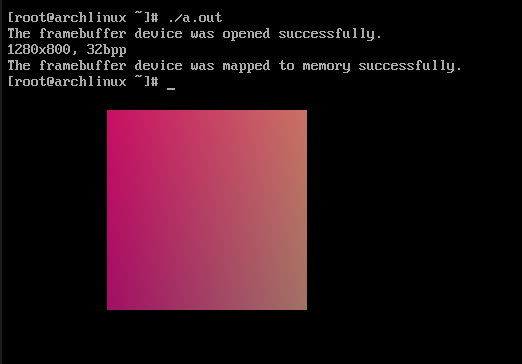
\includegraphics[scale=0.7]{realisierung/images/framebuffer-rectangle.png}
  \caption{C Programm welches einen Quadrat mit Gradient direkt in den Framebuffer schreibt}
\end{figure}

Jedoch wird es komplizierter, wenn man auch Text anzeigen möchte, da man jeden Pixel manuell schreiben muss welches bei Sätzen wie ``System Verification Failed'' bereits sehr umständlich ist.\\
Deshalb ist eine bessere lösung nötig, eine Bibliothek die in den Framebuffer schreiben kann und alle Rendering funktionen abstrahiert. Die Bibliothek die ich benutzt habe ist Raylib, eine C bibliothek welche hauptsächlich für die Entwicklung von Spielen gedacht ist, jedoch, nicht wie andere Engines, keine besonderen Features hat, sondern jediglich verschiedene Aspekte wie Grafik, Physik und Audio abstrahiert. Glücklicherweise kann mit der Compilerflag \texttt{-DEGL\_NO\_X11} raylib so kompiliert werden, dass es direkt in den Framebuffer schreibt, anstatt versucht ein Fenster zu öffnen.
\bigbreak \noindent
\begin{figure}[h]
  \centering
  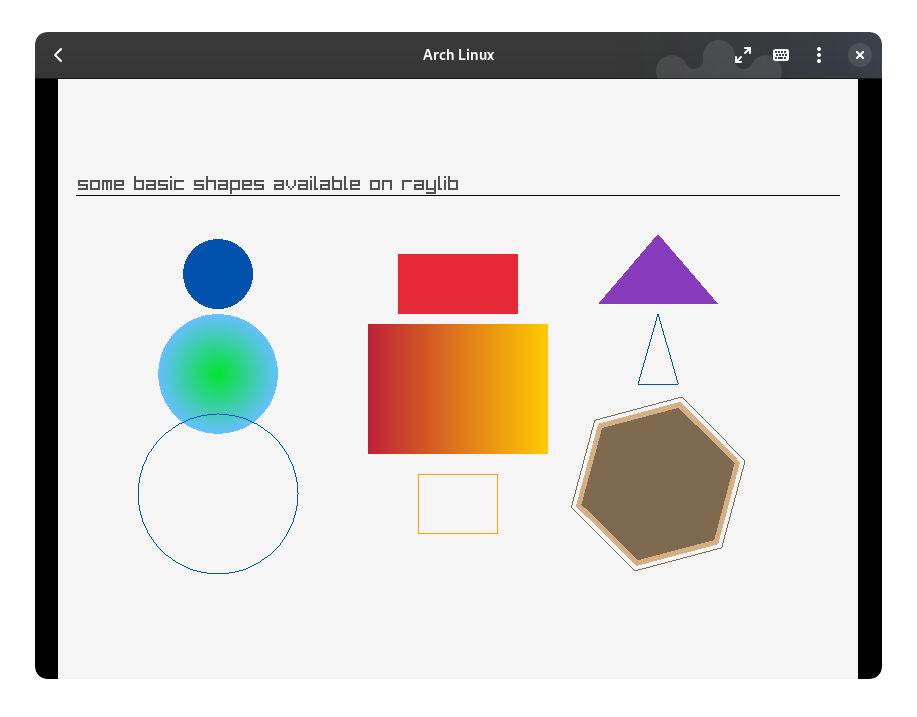
\includegraphics[scale=0.5]{realisierung/images/raylib-framebuffer.png}
  \caption{Raylib Beispielprogramm \texttt{shapes\_basic\_shapes} in einer VM mit output direkt zum Framebuffer}
\end{figure}

Hiermit wird es um einiges Einfacher eigene Bilder zu erstellen, die angezeigt werden wenn nötig.

\subsubsection{Grafikformat}
Da es recht umständlich wär, das Bild immer manuell in C zu programmieren, ist es am besten ein Grafikformat zu benutzen welches extern geladen werden kann. Der erste gedanke wäre, einfach jpg-xl oder png bilder zu benutzen, jedoch sind Rasterbasierte Grafikformate hier nicht sehr nützlich, da die Warnung auf viele verschiedene Bildschirmgrößen angezeigt werden muss, also sind Vektorbasierten Grafikformate nötig. Die bekannteste wäre SVG, eine XML basiertes Format mit dem Bilder geschrieben werden können, die unendlich groß skaliert werden können. SVG ist jedoch sehr komplex und hat features die hier nicht nötig sind.\\
Da ich kein Vektorbasiertes Grafikformat gefunden habe, welches auch sehr Simpel gehalten ist, habe ich mich entschlossen ein eigenes Format zu entwickeln.\\
\\
Das Format hat eine Funktionsbasierte Syntax, das heißt, dass im gegensatz zu SVG man einfach Funktionen aufruft um Formen zu zeichen oder Text zu schreiben:
\begin{verbatim}
rectangle (x=100,y=100,height=100,width=100,color="#FFFFFFFF",fill=true)
\end{verbatim}
Da diese art von Syntax sehr simpel zu Parsen ist, kann es alles direkt in POSIX-C implementiert werden, ohne externe Bibliotheken verwenden zu müssen.\\
Der nächste Schritt ist festzulegen, welche Funktionen benötigt werden. Mit betracht auf die Unterstützten Funktionen in raylib, habe ich die folgenden Funktionen implementiert:
\begin{itemize}
\item IMG\\
  Funktion um ein Bild zu Initialisieren, muss immer die erste Funktion in einem Bild sein.
\item rectangle\\
  Funktion um ein Rechteck zu zeichnen, unterstützt ausegfüllte und nicht ausgefüllte Rechtecke.
\item roundedrectangle\\
  Ein Rechteck aber mit abgerundeten Ecken.
\item circle\\
  Ein Kreis.
\item circlesegment\\
  Ein Kreissegment.
\item ring\\
  Ein Ring, kann genutzt werden um nicht ausegfüllte Kreise zu zeichnen.
\item ellipse\\
  Eine Ellipse.
\item triangle\\
  Ein Dreieck.
\item text\\
  Text.
\end{itemize}
Mit diesen Funktionen kann eine Bild ungefähr so aussehen:\\

\begin{verbatim}
// The IMG function is always required
// it initializes the image with its size
IMG (height=100, width=100)

// A rectangle 
rectangle (x=0, y=0, height=100, width=100, color="#5BCEFA", fill=true, thickness=0)

/*
 Rectangle but multiline
*/
rectangle (x=20, y=0,
height=60, width=100,
color="#F5A9B8",
fill=true, thickness=0)

circle (x=100,y=100,radius=10,color="#CfCfCf")
\end{verbatim}
Trotz des sehr simplen Aufbaus und kleinen Arsenal an Funktionen, ist es möglich viele verschiedene Dinge zu zeichnen, Perfekt um Grafiken für die Warnung von Nutzern zu erstellen.

\hypersetup{pageanchor=false}
\begin{figure}[h]
  \centering
  \begin{minipage}[c]{0.4\linewidth}
    
\includegraphics[width=\linewidth]{realisierung/images/bvg-haskell.png}
    \caption{Haskell Logo in bvg}
  \end{minipage}
  \hfill
  \begin{minipage}[c]{0.4\linewidth}
    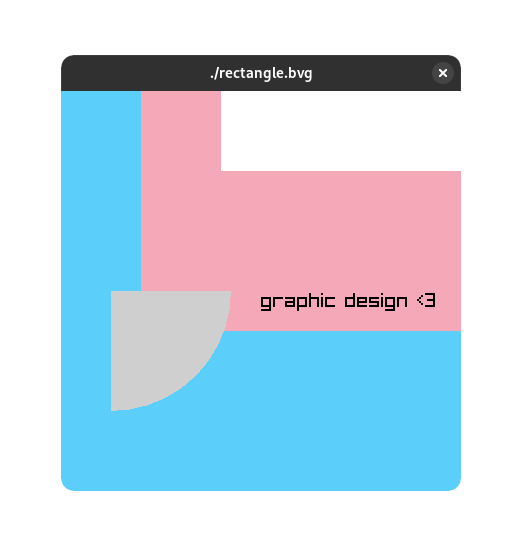
\includegraphics[width=\linewidth]{realisierung/images/bvg-rectangle.png}
    \caption{Rechtecke und Text}
  \end{minipage}
\end{figure}
\hypersetup{pageanchor=true}


%%% Local Variables:
%%% mode: LaTeX
%%% TeX-master: "../fsverify"
%%% End:


\section{Reflexion}
Insgesamt gibt es keine großen mängel, die mir während der Implementierung aufgefallen sind, die meisten Kritikpunkte liegen in fbwarn, welche teilweise der kurzen Entwicklungszeit (~7 Tage) zu schulden sind. 

\subsection{Bessere Datenbank}
Die Datenbank welche ich zurzeit nutze, bbolt, hat mehrere Probleme, zum einen ist die Lese und Schreibgeschwindigkeit nicht sehr schnell, trotz bestmöglicher Optimierungen durch nutzen von Batch-operations und einmaligen öffnen und Schreiben der Datenbank, fügt die Datenbank ungefähr 2 Sekunden an Laufzeit zu verifysetup, 22\% der ganzen Laufzeit.\\
Dazu kommt auch, das bbolt es zurzeit nicht unterstützt, eine Datenbank direkt aus einer Variable zu lesen, die Datenbank muss als Pfad im Dateisystem angegeben werden, welches dazu führt, das fsverify die Datenbank von der Partition in eine Variable liest, und die Variable direkt wieder in einer Datei in \texttt{/tmp} schreibt. Dies führt zu unnötigen Write-cycles die durch das Verwenden einer anderen Datenbank oder einem Patch für den bbolt Quellcode gelöst werden könnte.

\subsection{Nutzung vom TPM2 für öffentliche Schlüssel}
Dieses Feature war geplant, und ich hatte bereits einen Schlüssel durch verschiedene Linux Tools in den TPM geschrieben, jedoch konnte ich keine gute go Bibliothek für TPMs finden, weshalb ich das Feature auslassen musste, hätte ich dies noch bevore ich mit der Implementierung gewusst, hätte ich entweder eine andere Programmiersprache für fsverify gewählt, oder eine eigene Bibliothek für TPMs als teil des Projekts entwickelt.

\subsection{Besserer Parser für fbwarn}
Zur zeit benutzt fbwarn einfaches string matching mit Funktionen aus \texttt{stdlib.h} und \texttt{strings.h}, dies Funktioniert, jedoch bringt es viele Probleme mit sich, sodass zum Beispiel ein Leerzeichen am falschen Platz bereits vieles Zerstören kann, welches sehr schwer zu debuggen ist, da man Fehler solcher art nicht sofort erkennt.\\
Hätte ich mir für fbwarn mehr Zeit gegeben, hätte ich Programme benutzt, die Speziell für das Parsen von Dateien in C gedacht sind, wie \texttt{yacc(1)} und \texttt{lex(1)}.

\subsection{Mehr Funktionen in bvg}
bvg unterstützt zurzeit neun Funktionen, wie bereits gezeigt ist dies zwar genug um recht viel zu Zeichnen, jedoch unterstützen die Funktionen alle nur solide Farben, also keine Farbübergänge oder ähnliches, welches das Design der Bilder einschränkt und rehc ``alt'' erscheinen lässt, da Farbübergänge für elemente wie Schatten in modernen Designs sehr oft genutzt werden.\\
Zudem unterstützt bvg keinen Bézier Kurven, die das Zeichnen von beinahe jeder Form erlauben. Das fehlen ist jedoch ein Zeitproblem, da raylib bereits Funktionen für Bézier Kurven hat und die Implementierung in bvg recht simple wäre.

\bigbreak
\newpage

\includegraphics{by-sa.pdf}\\
This Document is licensed under CC-BY-SA 4.0. To view a copy of this license, visit\\
\url{https://creativecommons.org/licenses/by-sa/4.0/}\\
The source for this document can be found at\\ \url{https://github.com/axtloss/fsverify/tree/main/doc/class-assignment}
\end{document}

%%% Local Variables:
%%% mode: LaTeX
%%% TeX-master: t
%%% End:

\subsection{verifysetup}
Nachdem fsverify vollständig implementiert war und alle Speicherkonzepte vollständig Entwickelt sind, braucht fsverify auch ein Programm um alles richtig aufzusetzen.\\
Das Programm muss eine Datenbank von Nodes anhand der zu verifizierenden Partition erstellen, den Header entsprechend Konfigurieren und alles auf eine Datei schreiben, die der Nutzer (oder eher Distribution Entwickler) auf die für fsverify vorgesehene Partition schreiben kann.

\subsubsection{Optimierung}
Genauso wie fsverify, benutzt verifysetup erstmal nur einen Thread um die Datenbank zu erstellen. Dies führte zu einer laufzeit von über 2 Stunden für 1gb.\\
Die schritte zur optimierung sind die gleichen wie bei fsverify. Jedoch verbesserte sich die Laufzeit um einiges bereits bei dem wechsel zu 2kb Blocks und sha1 hashing, von 2 Stunden zu einer Stunde.\\
Mit dem wechsel zu multithreading ging dies dann runter zu 19 Sekunden mit 12 Threads.
\\
Die Laufzeit von verifysetup verbesserte sich um 33846\% in einer Woche.
\begin{verbatim}
10.02.2024: fsverify setup takes 110minutes to complete for 1gb
optimizations: none

12.02.2024: fsverify setup takes 71minutes to complete for 1gb
optimizations: block size 2k, sha1 instead of sha256

12.02.2024: fsverify setup takes ~9.54 seconds to complete for 1gb with 12 threads
optimizations: block size 2k, sha1 instead of sha256,
               multithreaded, db batch operations

17.02.2024: fsverify setup takes ~19.50 seconds to complete for 1gb with 12 threads
optimizations: block size 2k, sha1 instead of sha256,
               multithreaded, db batch operations
unoptimizations: enable database signing, header generation,
                 fsverify partition generation
\end{verbatim}
%%% Local Variables:
%%% mode: LaTeX
%%% TeX-master: "../fsverify"
%%% End:


\subsection{fbwarn}
Falls die Festplattenverifizierung Fehlschlägt, muss der Nutzer gewarnt werden (es ist auch möglich das Gerät einfach auszuschalten, jedoch sollte dies aus UX gründen nicht gemacht werden).

\subsubsection{Grafischer Output}
Die Warnung ist am besten grafisch zu tun, jedoch gibt es keinen display server wie Wayland oder X11, deshalb muss direkt auf den Framebuffer /dev/fb* geschrieben werden, um graphischen Output zu zeigen.\\
Da jeder verfügbare framebuffer als /dev/fbX verfügbar ist, kann man ganz einfach die Datei öffnen und mit mmap manipulieren:

\begin{minted}[fontsize=\footnotesize]{c}
 // imports: stdlib, linux/fb.h, stdio
 int main()
 {
     int fbfd = 0;
     struct fb_var_screeninfo vinfo;
     struct fb_fix_screeninfo finfo;
     
     // Open the framebuffer file for reading and writing
     fbfd = open("/dev/fb0", O_RDWR);
          
     // Get fixed screen information
     ioctl(fbfd, FBIOGET_FSCREENINFO, &finfo);
     // Get variable screen information
     ioctl(fbfd, FBIOGET_VSCREENINFO, &vinfo);
  
     // Map the device to memory
     fbp = (char *)mmap(0, screensize, PROT_READ | PROT_WRITE, MAP_SHARED, fbfd, 0);
 
     location = (300+vinfo.xoffset) * (vinfo.bits_per_pixel/8) + \
                (100+vinfo.yoffset) * finfo.line_length;
     *(fbp + location) = 100;        // Some blue
     *(fbp + location + 1) = 50;     // A little green
     *(fbp + location + 2) = 200;    // A lot of red
     *(fbp + location + 3) = 0;      // No transparency

     munmap(fbp, screensize);
     close(fbfd);
     return 0;
 }
\end{minted}
Dies genügt, wenn man einfache Formen in den Framebuffer zeichnen möchte, wie im Bild zu sehen ist
\begin{figure}[h]
  \centering
  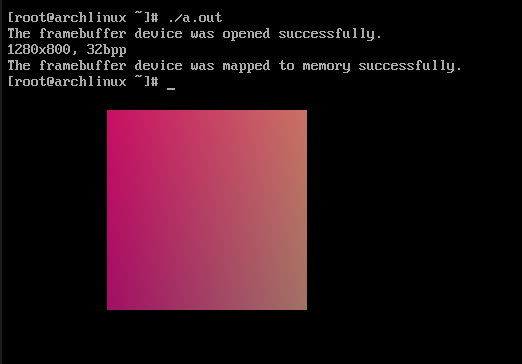
\includegraphics[scale=0.7]{realisierung/images/framebuffer-rectangle.png}
  \caption{C Programm welches einen Quadrat mit Gradient direkt in den Framebuffer schreibt}
\end{figure}

Jedoch wird es komplizierter, wenn man auch Text anzeigen möchte, da man jeden Pixel manuell schreiben muss welches bei Sätzen wie ``System Verification Failed'' bereits sehr umständlich ist.\\
Deshalb ist eine bessere lösung nötig, eine Bibliothek die in den Framebuffer schreiben kann und alle Rendering funktionen abstrahiert. Die Bibliothek die ich benutzt habe ist Raylib, eine C bibliothek welche hauptsächlich für die Entwicklung von Spielen gedacht ist, jedoch, nicht wie andere Engines, keine besonderen Features hat, sondern jediglich verschiedene Aspekte wie Grafik, Physik und Audio abstrahiert. Glücklicherweise kann mit der Compilerflag \texttt{-DEGL\_NO\_X11} raylib so kompiliert werden, dass es direkt in den Framebuffer schreibt, anstatt versucht ein Fenster zu öffnen.
\bigbreak \noindent
\begin{figure}[h]
  \centering
  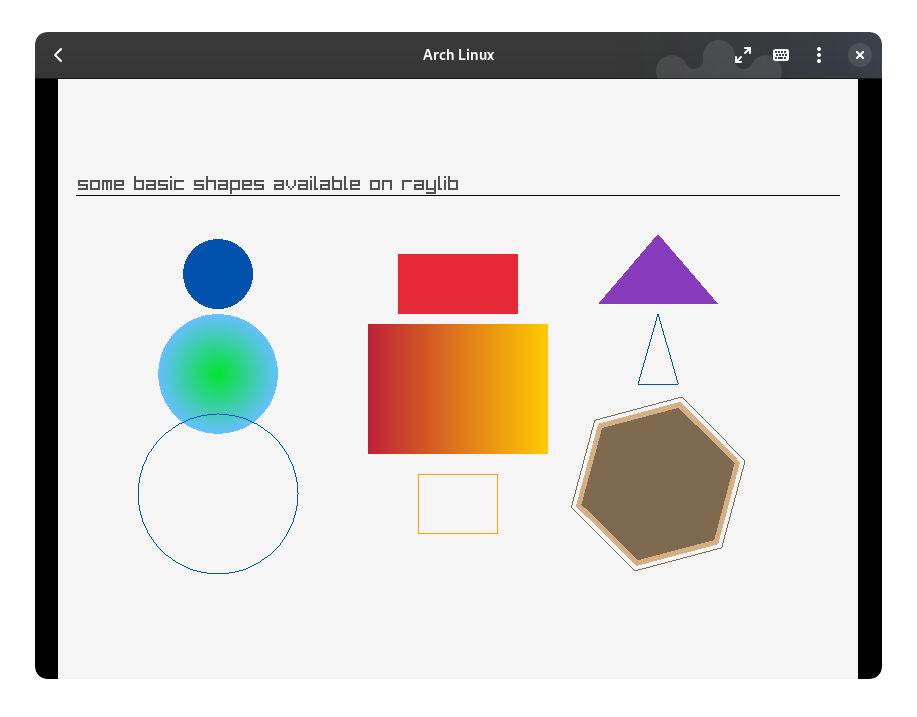
\includegraphics[scale=0.5]{realisierung/images/raylib-framebuffer.png}
  \caption{Raylib Beispielprogramm \texttt{shapes\_basic\_shapes} in einer VM mit output direkt zum Framebuffer}
\end{figure}

Hiermit wird es um einiges Einfacher eigene Bilder zu erstellen, die angezeigt werden wenn nötig.

\subsubsection{Grafikformat}
Da es recht umständlich wär, das Bild immer manuell in C zu programmieren, ist es am besten ein Grafikformat zu benutzen welches extern geladen werden kann. Der erste gedanke wäre, einfach jpg-xl oder png bilder zu benutzen, jedoch sind Rasterbasierte Grafikformate hier nicht sehr nützlich, da die Warnung auf viele verschiedene Bildschirmgrößen angezeigt werden muss, also sind Vektorbasierten Grafikformate nötig. Die bekannteste wäre SVG, eine XML basiertes Format mit dem Bilder geschrieben werden können, die unendlich groß skaliert werden können. SVG ist jedoch sehr komplex und hat features die hier nicht nötig sind.\\
Da ich kein Vektorbasiertes Grafikformat gefunden habe, welches auch sehr Simpel gehalten ist, habe ich mich entschlossen ein eigenes Format zu entwickeln.\\
\\
Das Format hat eine Funktionsbasierte Syntax, das heißt, dass im gegensatz zu SVG man einfach Funktionen aufruft um Formen zu zeichen oder Text zu schreiben:
\begin{verbatim}
rectangle (x=100,y=100,height=100,width=100,color="#FFFFFFFF",fill=true)
\end{verbatim}
Da diese art von Syntax sehr simpel zu Parsen ist, kann es alles direkt in POSIX-C implementiert werden, ohne externe Bibliotheken verwenden zu müssen.\\
Der nächste Schritt ist festzulegen, welche Funktionen benötigt werden. Mit betracht auf die Unterstützten Funktionen in raylib, habe ich die folgenden Funktionen implementiert:
\begin{itemize}
\item IMG\\
  Funktion um ein Bild zu Initialisieren, muss immer die erste Funktion in einem Bild sein.
\item rectangle\\
  Funktion um ein Rechteck zu zeichnen, unterstützt ausegfüllte und nicht ausgefüllte Rechtecke.
\item roundedrectangle\\
  Ein Rechteck aber mit abgerundeten Ecken.
\item circle\\
  Ein Kreis.
\item circlesegment\\
  Ein Kreissegment.
\item ring\\
  Ein Ring, kann genutzt werden um nicht ausegfüllte Kreise zu zeichnen.
\item ellipse\\
  Eine Ellipse.
\item triangle\\
  Ein Dreieck.
\item text\\
  Text.
\end{itemize}
Mit diesen Funktionen kann eine Bild ungefähr so aussehen:\\

\begin{verbatim}
// The IMG function is always required
// it initializes the image with its size
IMG (height=100, width=100)

// A rectangle 
rectangle (x=0, y=0, height=100, width=100, color="#5BCEFA", fill=true, thickness=0)

/*
 Rectangle but multiline
*/
rectangle (x=20, y=0,
height=60, width=100,
color="#F5A9B8",
fill=true, thickness=0)

circle (x=100,y=100,radius=10,color="#CfCfCf")
\end{verbatim}
Trotz des sehr simplen Aufbaus und kleinen Arsenal an Funktionen, ist es möglich viele verschiedene Dinge zu zeichnen, Perfekt um Grafiken für die Warnung von Nutzern zu erstellen.

\hypersetup{pageanchor=false}
\begin{figure}[h]
  \centering
  \begin{minipage}[c]{0.4\linewidth}
    
\includegraphics[width=\linewidth]{realisierung/images/bvg-haskell.png}
    \caption{Haskell Logo in bvg}
  \end{minipage}
  \hfill
  \begin{minipage}[c]{0.4\linewidth}
    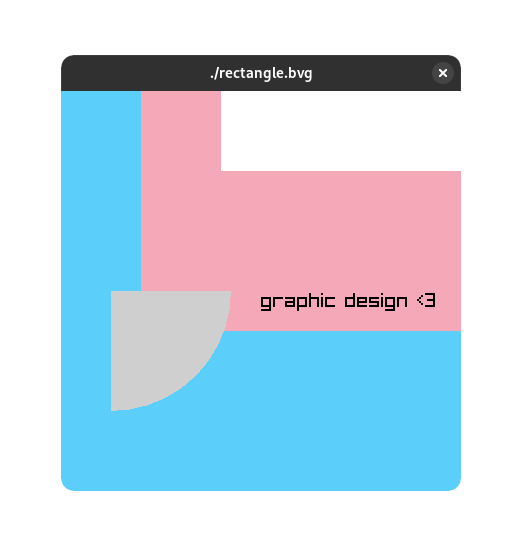
\includegraphics[width=\linewidth]{realisierung/images/bvg-rectangle.png}
    \caption{Rechtecke und Text}
  \end{minipage}
\end{figure}
\hypersetup{pageanchor=true}


%%% Local Variables:
%%% mode: LaTeX
%%% TeX-master: "../fsverify"
%%% End:

